\chapter{Methodology}
\label{sec:methodology} 

\section{Data}
\label{sec:data}

\subsection{Real Dataset}
\label{sec:ch4_realdata}
To evaluate the performance of dPCR droplet classifiers, a publicly available dataset from the study of \citeA{Lievens2016} was analyzed. Their premise is that there was no established criteria to assess dPCR assay quality; they addressed this problem in their study by proposing measures to evaluate the following criteria: i.) there should only be a single amplification product (i.e. only two fluorescence population is present), ii.) clear separation between positive and negatives, iii.) and limit the amount of intermediate fluorescence. Having set these standards, \shortciteauthor{Lievens2016} designed nine plates, or sets, of experimental parameters in aims of optimizing their own dPCR samples. They have examined twelve DNA targets from stock solutions of food and feed materials. In the first plate, reaction mixes were prepared using real-time qPCR validated conditions, this resulted in poor dPCR performance metrics. To improve the results, they experimented on experimental parameters that were proven effective in other studies. The list of the experimental factors explored are shown in [TABLE 1]. In plates 1 and 9, the experimental factors were already fixed. As for the other plates, varying levels of the specified factors were ran as a means of finding the optimal parameter. It can be seen that two DNA targets (TC1507 and M88017) were closely examined for half of the plates, this is due to the fact that both were producing significant amounts of rain. In fact, most of the samples prepared were exhibiting noise characteristics. The observed dPCR quality for each plate is summarized in [TABLE 2].  

% [Table 1]
\begin{table}
    \centering
    \small
    \caption{Levels of the design factors per plate and the DNA targets examined}
    \begin{tabular}{lllllll} 
    \toprule
    \begin{tabular}[c]{@{}l@{}}\textbf{Plate – Experimental}\\\textbf{Factor }\end{tabular} & \multicolumn{2}{l}{\textbf{Levels }} & \multicolumn{4}{l}{\textbf{DNA Targets }} \\ 
    \midrule
    \multirow{4}{*}{\begin{tabular}[c]{@{}l@{}}1 - qPCR validated\\conditions \end{tabular}} & \multicolumn{2}{l}{\multirow{4}{*}{N/A}} & \vcell{acp} & \multicolumn{2}{l}{\vcell{hmg}} & \vcell{M88017} \\[-\rowheight]
     & \multicolumn{2}{l}{} & \printcellmiddle & \multicolumn{2}{l}{\printcellmiddle} & \printcellmiddle \\
     & \multicolumn{2}{l}{} & cru & \multicolumn{2}{l}{le1} & M88701 \\
     & \multicolumn{2}{l}{} & GT73 & \multicolumn{2}{l}{M1445} & M89788 \\
     & \multicolumn{2}{l}{} & GTS4032 & \multicolumn{2}{l}{M810} & TC1507 \\ 
    \cmidrule(r){1-7}
    \multirow{4}{*}{\begin{tabular}[c]{@{}l@{}}2 – Primer\\concentration \end{tabular}} & \multirow{2}{*}{150} & \multirow{2}{*}{450} & \vcell{acp} & \multicolumn{2}{l}{\vcell{hmg}} & \vcell{M88017} \\[-\rowheight]
     &  &  & \printcellmiddle & \multicolumn{2}{l}{\printcellmiddle} & \printcellmiddle \\
     &  &  & cru & \multicolumn{2}{l}{le1} & M88701 \\
     & \multirow{2}{*}{300} & \multirow{2}{*}{600} & GT73 & \multicolumn{2}{l}{M1445} & M89788 \\
     &  &  & GTS4032 & \multicolumn{2}{l}{M810} & TC1507 \\ 
    \cmidrule(lr){1-7}
    \multirow{3}{*}{\begin{tabular}[c]{@{}l@{}}3 - Two-fold dilution \\series \end{tabular}} & \vcell{Conc 8000} & \vcell{Conc 1000} & \multicolumn{2}{l}{\multirow{3}{*}{M88701}} & \multicolumn{2}{l}{\multirow{3}{*}{TC1507}} \\[-\rowheight]
     & \printcellmiddle & \printcellmiddle & \multicolumn{2}{l}{} & \multicolumn{2}{l}{} \\
     & Conc 4000 & Conc 500 & \multicolumn{2}{l}{} & \multicolumn{2}{l}{} \\
     & Conc 2000 & Conc 250 & \multicolumn{2}{l}{} & \multicolumn{2}{l}{} \\ 
    \cmidrule(lr){1-7}
    \multirow{3}{*}{4 - PCR Enhancers} & \multicolumn{2}{l}{\vcell{Enhancer NA (none)}} & \multicolumn{2}{l}{\multirow{3}{*}{M88701}} & \multicolumn{2}{l}{\multirow{3}{*}{TC1507}} \\[-\rowheight]
     & \multicolumn{2}{l}{\printcellmiddle} & \multicolumn{2}{l}{} & \multicolumn{2}{l}{} \\
     & \multicolumn{2}{l}{Enhancer DMSO2\%} & \multicolumn{2}{l}{} & \multicolumn{2}{l}{} \\
     & \multicolumn{2}{l}{Enhancer Trehalose0.2M} & \multicolumn{2}{l}{} & \multicolumn{2}{l}{} \\ 
     \cmidrule(lr){1-7}
    \multirow{8}{*}{\begin{tabular}[c]{@{}l@{}}5 - Two-fold dilution \\and Cycles \end{tabular}} & \multicolumn{2}{l}{\vcell{Conc 8000 Cycles 45}} & \multicolumn{2}{l}{\multirow{8}{*}{M88701}} & \multicolumn{2}{l}{\multirow{8}{*}{TC1507}} \\[-\rowheight]
     & \multicolumn{2}{l}{\printcellmiddle} & \multicolumn{2}{l}{} & \multicolumn{2}{l}{} \\
     & \multicolumn{2}{l}{Conc 8000 Cycles 60} & \multicolumn{2}{l}{} & \multicolumn{2}{l}{} \\
     & \multicolumn{2}{l}{Conc 8000 Cycles 75} & \multicolumn{2}{l}{} & \multicolumn{2}{l}{} \\
     & \multicolumn{2}{l}{Conc 8000 Cycles 90} & \multicolumn{2}{l}{} & \multicolumn{2}{l}{} \\
     & \multicolumn{2}{l}{Conc 4000 Cycles 45} & \multicolumn{2}{l}{} & \multicolumn{2}{l}{} \\
     & \multicolumn{2}{l}{Conc 4000 Cycles 60} & \multicolumn{2}{l}{} & \multicolumn{2}{l}{} \\
     & \multicolumn{2}{l}{Conc 4000 Cycles 75} & \multicolumn{2}{l}{} & \multicolumn{2}{l}{} \\
     & \multicolumn{2}{l}{Conc 4000 Cycles 90} & \multicolumn{2}{l}{} & \multicolumn{2}{l}{} \\ 
     \cmidrule(lr){1-7}
    \multirow{3}{*}{6 – Sonication time} & \vcell{0} & \vcell{9} & \multicolumn{2}{l}{\multirow{3}{*}{M88701}} & \multicolumn{2}{l}{\multirow{3}{*}{TC1507}} \\[-\rowheight]
     & \printcellmiddle & \printcellmiddle & \multicolumn{2}{l}{} & \multicolumn{2}{l}{} \\
     & 3 & 12 & \multicolumn{2}{l}{} & \multicolumn{2}{l}{} \\
     & 6 & 15 & \multicolumn{2}{l}{} & \multicolumn{2}{l}{} \\ 
     \cmidrule(lr){1-7}
    \multirow{4}{*}{\begin{tabular}[c]{@{}l@{}}7 - Annealing \\temperature \end{tabular}} & \vcell{62} & \vcell{58.4} & \vcell{acp} & \multicolumn{2}{l}{\vcell{hmg}} & \vcell{M88017} \\[-\rowheight]
     & \printcellmiddle & \printcellmiddle & \printcellmiddle & \multicolumn{2}{l}{\printcellmiddle} & \printcellmiddle \\
     & 61.6 & 57.3 & cru & \multicolumn{2}{l}{le1} & M88701 \\
     & 60.9 & 56.5 & GT73 & \multicolumn{2}{l}{M1445} & M89788 \\
     & 59.8 & 56 & GTS4032 & \multicolumn{2}{l}{M810} & TC1507 \\ 
    \cmidrule(lr){1-7}
    \multirow{4}{*}{\begin{tabular}[c]{@{}l@{}}9 - dPCR optimized \\parameters \end{tabular}} & \multicolumn{2}{l}{\multirow{4}{*}{N/A}} & \vcell{GT73} & \multicolumn{2}{l}{\vcell{M1445}} & \vcell{M89788} \\[-\rowheight]
     & \multicolumn{2}{l}{} & \printcellmiddle & \multicolumn{2}{l}{\printcellmiddle} & \printcellmiddle \\
     & \multicolumn{2}{l}{} & GTS4032 & \multicolumn{2}{l}{M810} & TC1507 \\
     & \multicolumn{2}{l}{} & hmg & \multicolumn{2}{l}{M88017} &  \\
     & \multicolumn{2}{l}{} & le1 & \multicolumn{2}{l}{M88701} &  \\ 
     \bottomrule
     &  &  &  &  &  & 
    \end{tabular}
\end{table}

% [Table 2]
\begin{table}
    \small	
    \caption{Observed assay quality results per experimental factor}    
    \begin{tabularx}{\textwidth}{p{2.7cm}*{3}{X}}
        \toprule
        \textbf{Plate – \newline Experimental Factor}       & \textbf{Lievens et.al’s remarks on the results}                                                                                                                                                                             & \textbf{Additional remarks from our   observations}                                                                                                                                                \\ 
        \midrule
        \arrayrulecolor[rgb]{0.753,0.753,0.753}
        1 - qPCR validated condition     & - More than two populations  amplified  for acp and cru \newline - High amount of rain for TC1507  and M88017                                                                      & - Negligible amount of rain for few   targets \newline - Moderate amount of rain for few targets \\
        \hline
        2 - Primer concentration         & - Significant increase in peak   separation at higher primer concentrations                                                                                                                                                 & - No effect for some targets                                                                                                                                                                       \\
        \hline
        3 - Two-fold dilution series     & - Rain is concluded to contain   target sequence but does not amplify at the same efficiency as the distinct   positives                                                                                                    & - Moderate amount of rain at higher   concentrations for both targets                                                                                                                              \\
        \hline
        4 - PCR Enhancers                                                                  & - No effect for both targets                                                                                                                                                                                                & - More than two populations amplified for   one replicate of M88017                                                                                                                                \\
        \hline
        5 - Two-fold dilution and Cycles  & - Rain is decreased at higher   cycles for both targets                                                                                                                                                                     &                                                                                                                                                                                                    \\
        \hline
        6 - Sonication                                                                     & - Significant decrease in rain for   M88017 \newline - No effect for TC1507                                                                                                          &                                                                                                                                                                                                    \\
        \hline
        7 - Annealing temperature        & - Significant increase in peak   separation at higher temperatures for TC1507 and GTS4032 \newline - Increased rain at higher   temperatures \newline - No effect for cru and MON1445 & - High presence of rain for some   targets \newline - More than two populations   amplified for acp and cru \newline- Two populations overlap for   GTS4032 \\
        \hline
        9 - dPCR optimized parameters     & - Optimal peak separation, template   DNA concentration, and at most 2.5\% rain* for all targets.                                                                                                                           & - More than two populations   amplified for one replicate of M88701 \newline - Moderate amount of rain for some   targets                                   \\
        \arrayrulecolor{black}
        \bottomrule    
    \end{tabularx}
\end{table}

\begin{figure}[h]
    \centering
    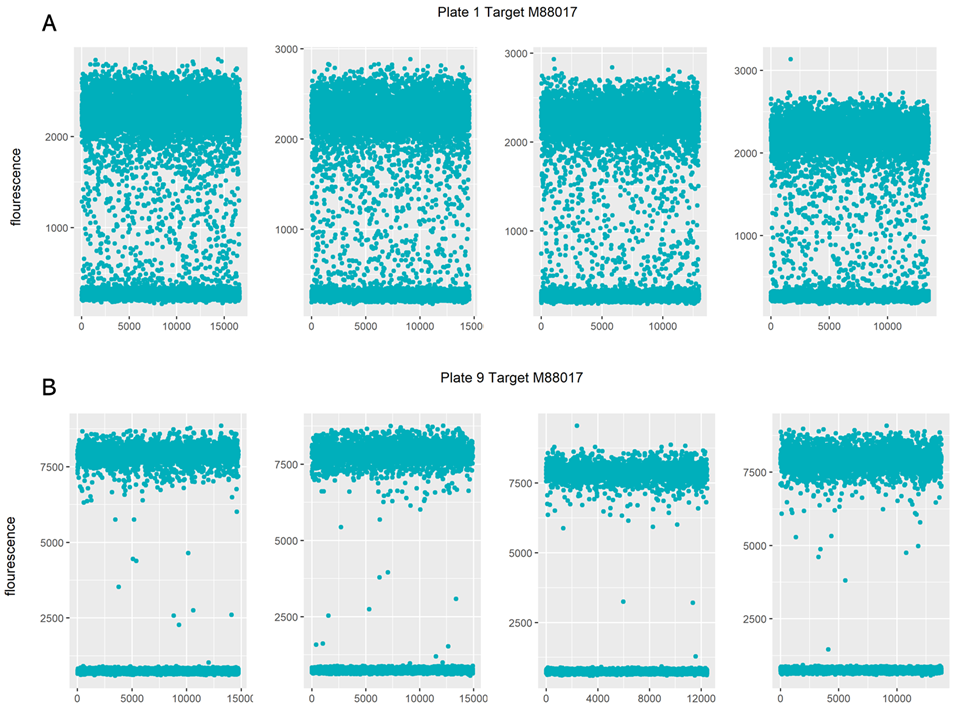
\includegraphics[max size={\textwidth}{\textheight}]{samplepreview_optimized.png}
    \caption[Lieven's optimization results for target M88017]%
    {Lieven's optimization results for target M88017- (A) Using real-time qPCR validated design parameters, target M88017 displays very ambiguous readouts. (B) Using the same target but with optimized dPCR parameters, it can be seen that there is significant reduction of rain and increased separation between the two populations.}
     \label{fig:samplepreview_optimized}
\end{figure}

For DNA target M88017 in figure \ref{fig:samplepreview_optimized}, it is visually obvious that from the initial qPCR validated conditions (subfigure A) their dPCR assay optimization (subfigure B) has been effective in clearing out the rain and also in separating the two populations. However, it should be noted that this is not the case for all the targets, as some still exhibit an amount of rain fluorescence in their optimized parameters. In contrast, figure \ref{fig:samplepreview_bad} demonstrates selected samples with noisy features. All the sample replicates in plate 1 acp (subfigure A) produces more than 2 bands of fluorescence intensities. In plate 4 where PCR Enhancers were noted to be not effective, each of the target M88017 samples with no enhancer, DMS20\%, and trehalose enhancer (subfigure B) can be seen to produce heavy rain. In the case of target M88017 in plate 6 (subfigure C), it can be observed that applying sonication reduced the rain droplets. Although it is impossible to have all the \(\lambda\) estimate to be equal within a sample, since DNA extraction was from the organism, it is expected to some degree that the estimates should be very close to each other, regardless of the presence of noise.

\begin{figure}[h]
    \centering
    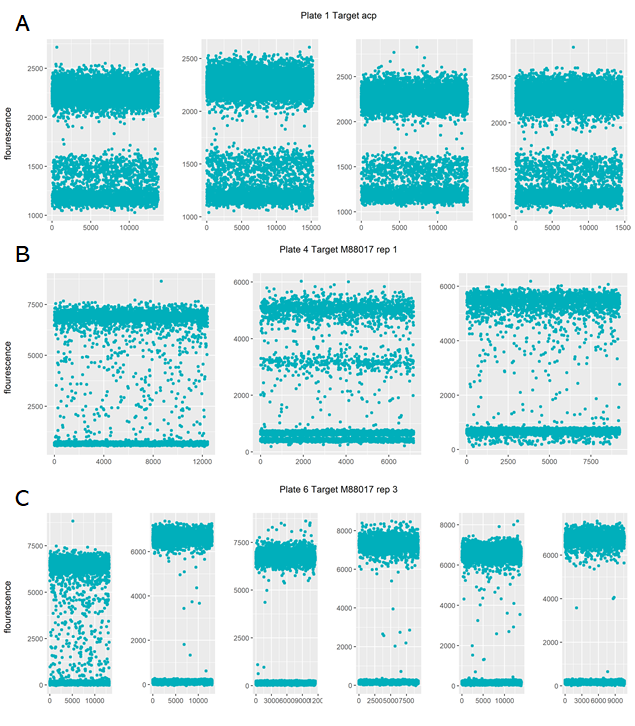
\includegraphics[max size={\textwidth}{\textheight}]{samplepreview_bad.png}
    \caption[Example dPCR results using different experimental factors]%
    { Example dPCR results using different experimental factors- (A) Target acp using real-time qPCR validated condition. (B) Target M88017 with no PCR enhancers, DMSO20\% enhancer, and trehalose enhancer (one replicate each from left to right). (C) Target M88017 with sonication 0, 3, 6, 9, 12, and 15 (one replicate each from left to right).}
     \label{fig:samplepreview_bad}
\end{figure}

\subsection{Simulated Dataset}
\label{sec:simdataset}
For this study, it is also of interest to assess the performance of droplet classifiers in extreme cases of dPCR assay quality. Since the real dataset from the previous section only has a few samples exhibiting significant amount of rain and poor separation of populations, a dataset with these characteristics were simulated. This section first reviews the simulation settings of \citeA{Jacobs2017}, and then describes the common and unique features of this study's simulation procedure.

In an attempt to explore the accuracy of their concentration estimator in various noise levels, \shortciteauthor{Jacobs2017} simulated 9 rain settings of 4 different concentrations. For each rain and concentration setting, 15 replicates of target samples and 3 replicates of NTC samples were generated. The middle facet in figure \ref{fig:jacobssim} displays a target sample for each setting. The columns from left to right simulates the concentrations \(\lambda = 0.1, 0.4, 1, 2.5\) (also indicated as blue, pink, red, and yellow, respectively). The rows from top to bottom simulates very minimal to high amounts of rain amplified by the increasing overlap of the two fluorescence populations. Results are summarized in the left and right facet in figure \ref{fig:jacobssim}, where for each rain and concentration setting, the distribution of \(\lambda\) point estimates should ideally be very close to the true \(\lambda\) values (colored horizontal line).

\begin{figure}[h]
    \centering
    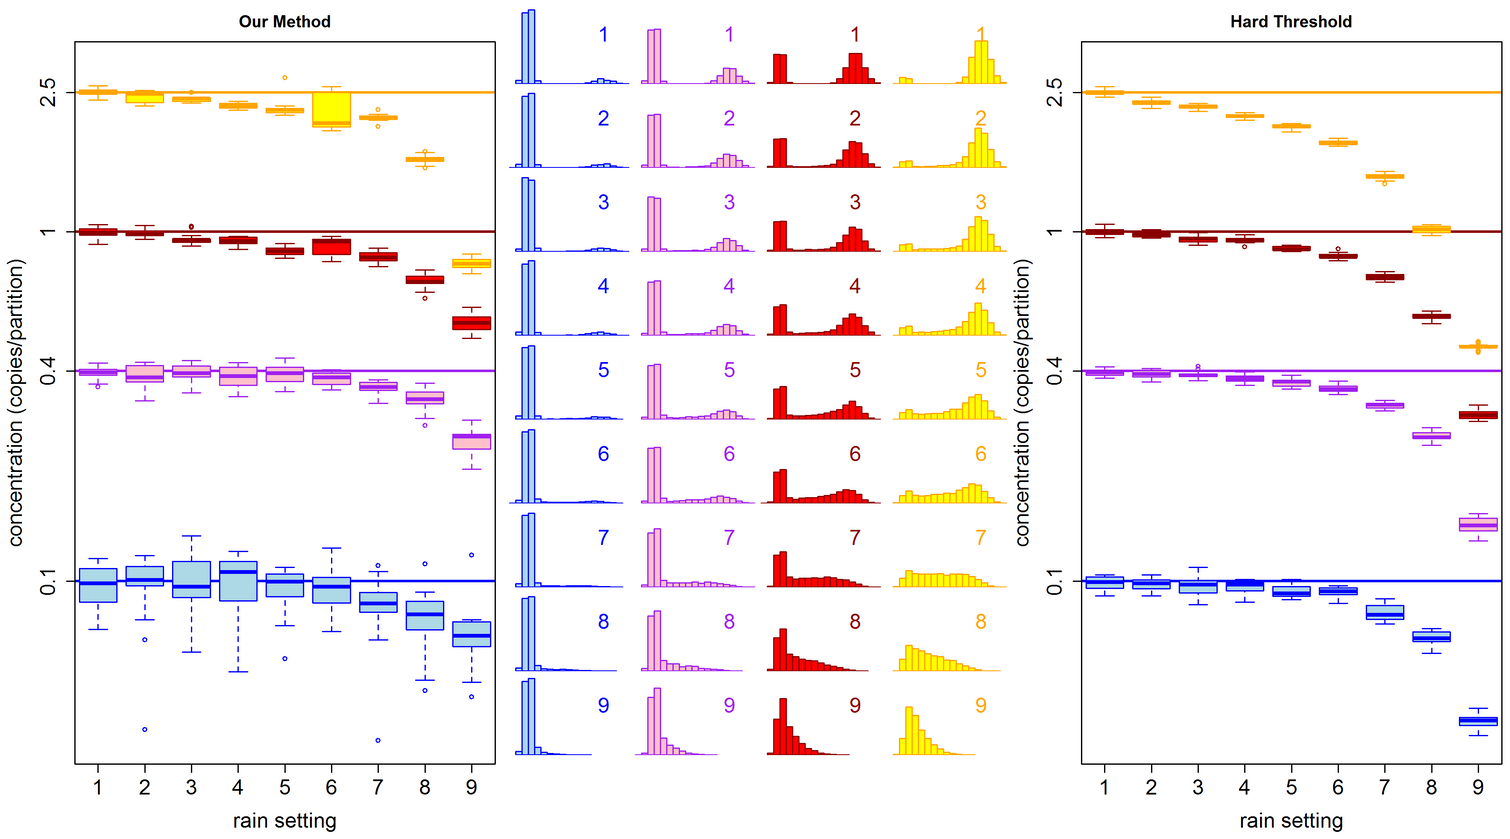
\includegraphics[max size={\textwidth}{\textheight}]{jacobssim.png}
    \caption[Simulated data and accuracy results from Jacobs et. al]{Simulated data and accuracy results from Jacobs et. al- Reprinted from Jacobs, Bart K. M.; Goetghebeur, Els; Vandesompele, Jo; De Ganck, Ariane; Nijs, Nele; Beckers, Anneleen; et al. (2017): Model-Based Classification for Digital PCR: Your Umbrella for Rain. ACS Publications. Collection. https://doi.org/10.1021/acs.analchem.6b04208}
        \label{fig:jacobssim}
\end{figure}

This experiment allowed them to compare the accuracy of quantification methods in extreme cases of clean and noisy data. However, since this dataset nor the code to reproduce it is not publicly available, other researchers who may want to compare their method using the same settings may have to simulate their own.

Selected features of the simulation of \citeA{Jacobs2017} were reproduced for this study. A dataset of varying rain levels and concentrations were generated with 4 rain settings (No rain, Low rain, Moderate ran, and High rain) and 5 concentration levels (\(\lambda = 0.1, 0.2236, 0.5, 1.118, 2.5\)). The concentration range of 0.1 - 2.5  was based on \citeA{Jacobs2017}, but the values in between was modified to be a geometric sequence to mimic a dilution series. Likewise, 15 replicates of target samples and 3 replicates of NTC samples were generated. Figure \ref{fig:mysim} shows a replicate of an artificial dPCR droplet fluorescence for each setting.

\begin{figure}[h]
    \centering
    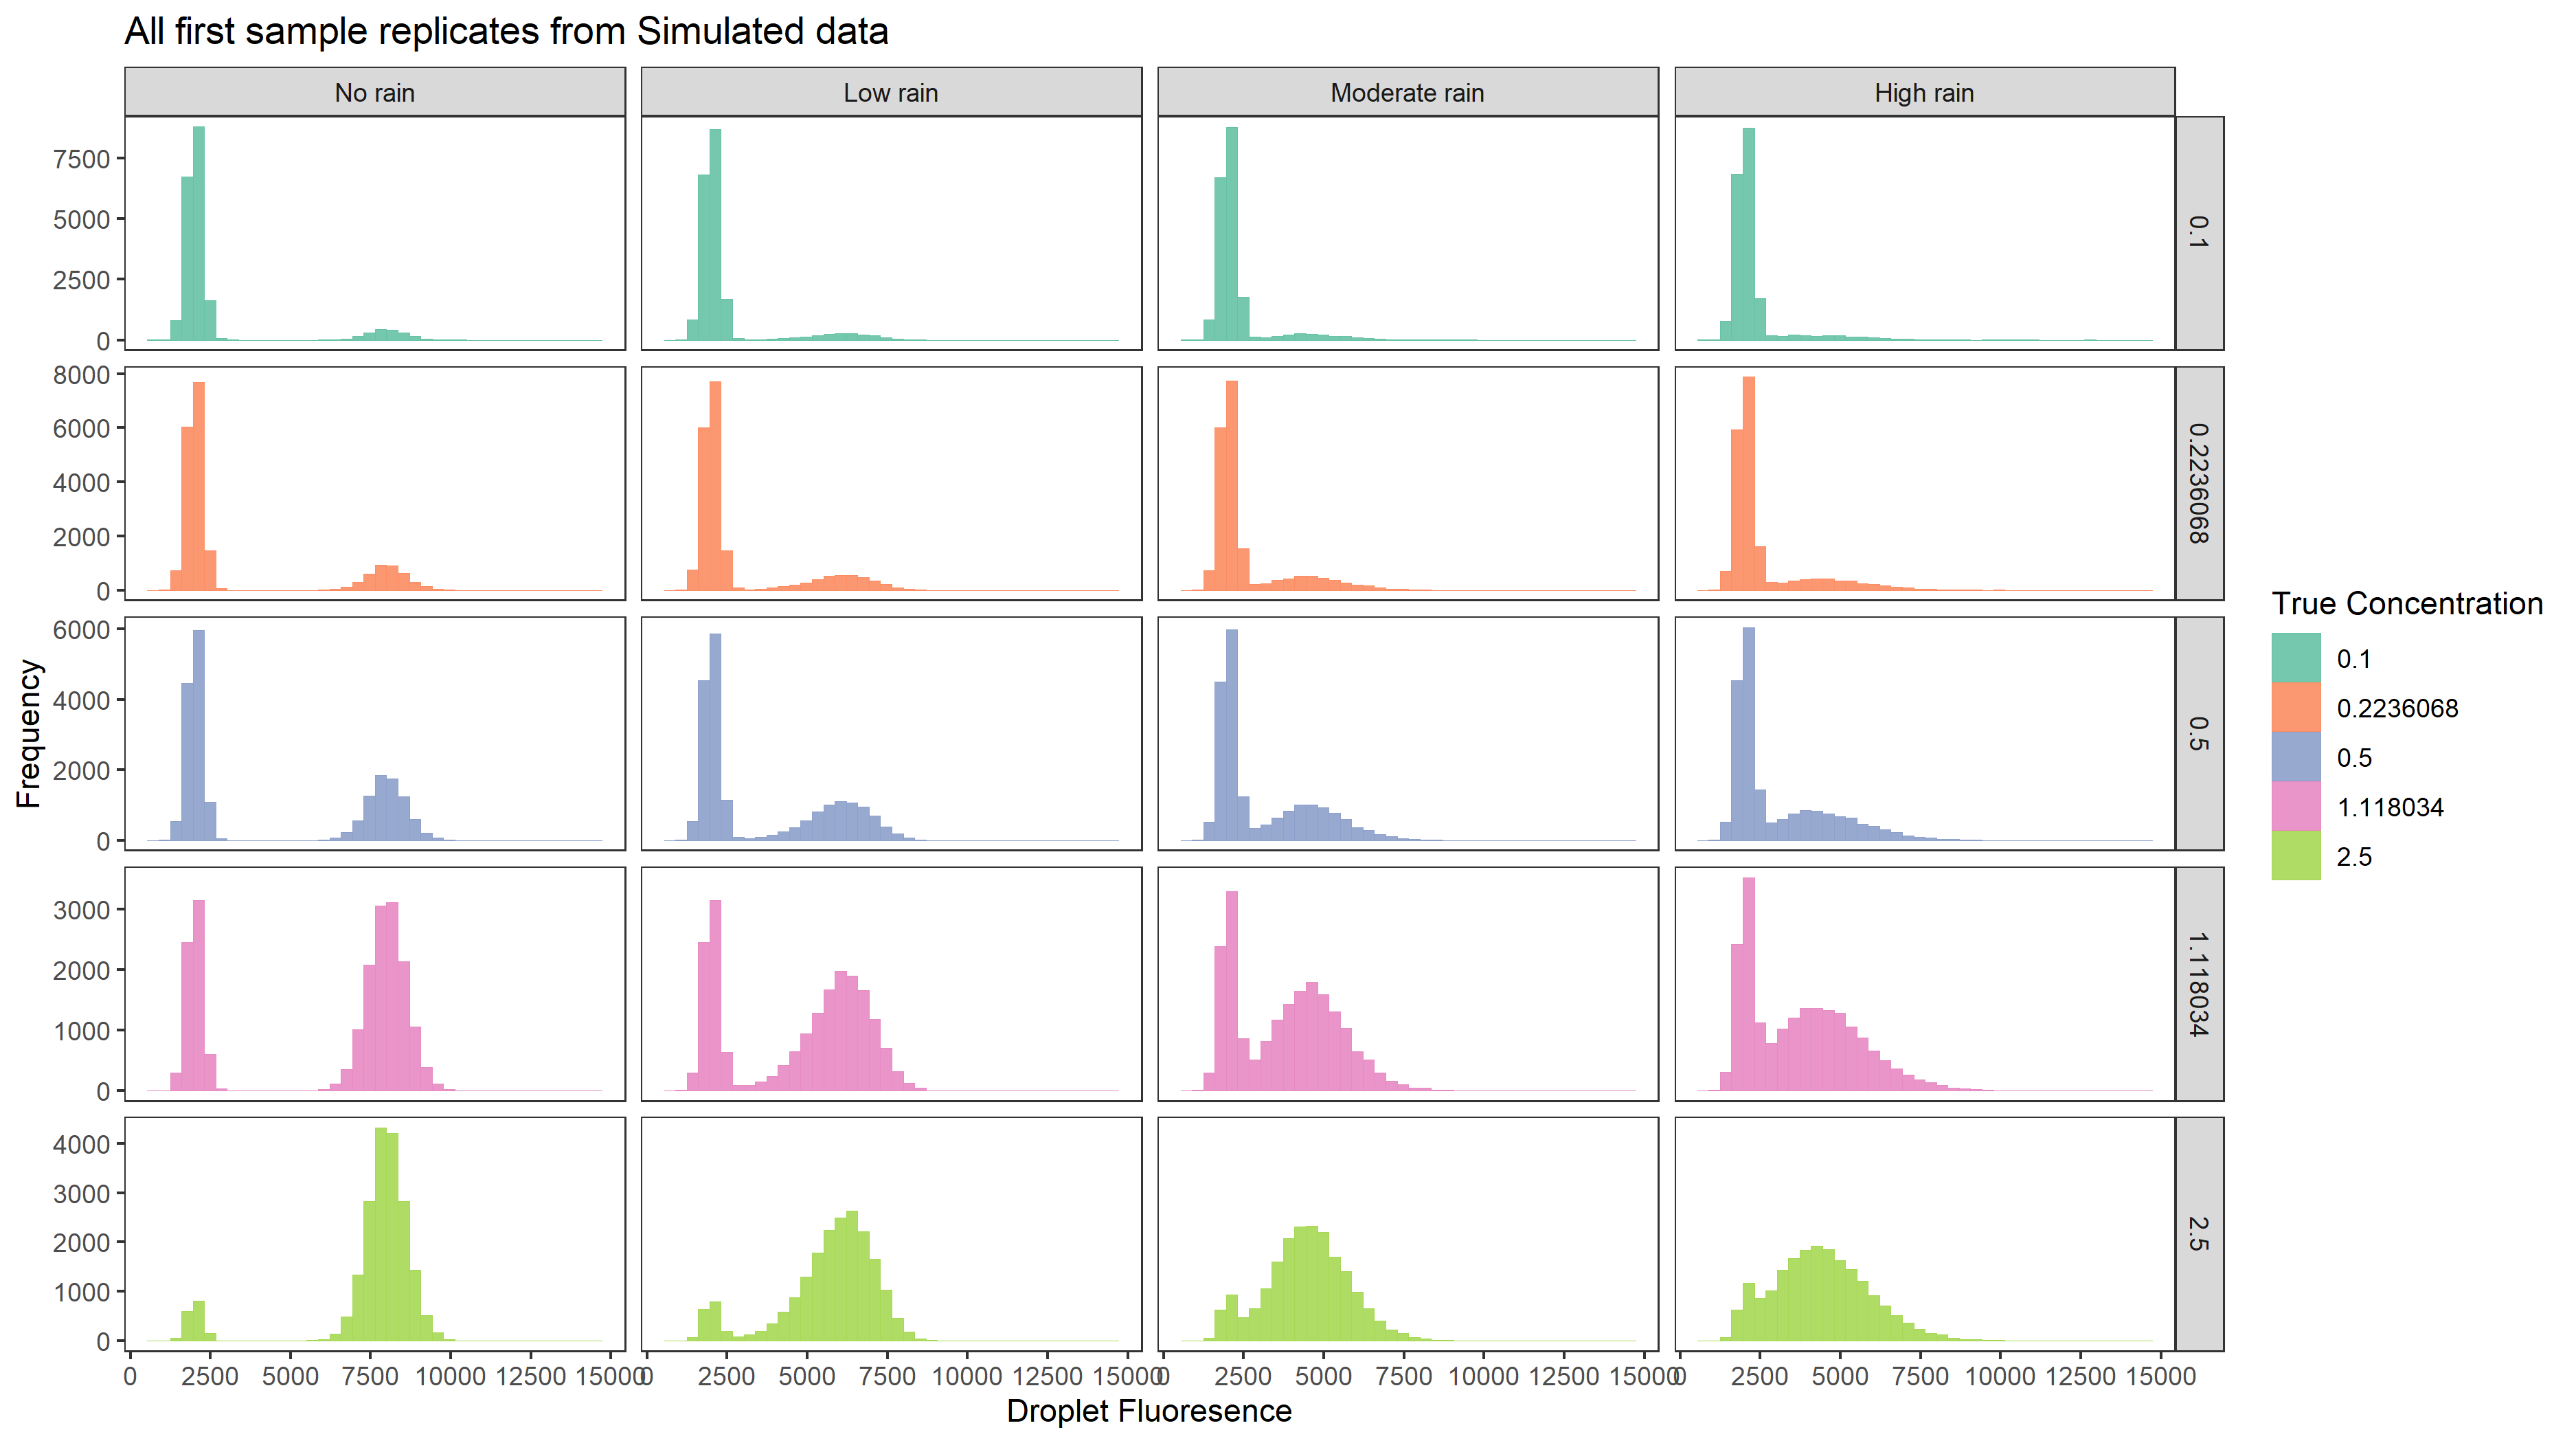
\includegraphics[max size={\textwidth}{\textheight}]{mysim.png}
    \caption[Simulated dataset for this study]{Simulated dataset for this study- Displayed are one sample replicates for each rain and concentration setting. Generated from fitting GH mixture models on real dPCR data.}
        \label{fig:mysim}
\end{figure}

In order to closely mimic the behaviour of real world data, selected dPCR assays from section \ref{sec:ch4_realdata} was fitted using a GH distribution mixture model. Observe in figure \ref{fig:realdata_gts} the fluorescence distribution of Plate 7 for target GTS4032. Each assay were ran in identical conditions but with different annealing temperatures (62, 61.6, 60.9, 59.8, 58.4, 57.3, 56.5, 56 \(^{\circ}\)C; from A to E). High presence of rain and poor separation of populations is obvious in grid A. These noise characteristics were slightly reduced in B; and in C, the separation of the populations improved. In contrast, H achieved a clear separation of the fluorescence populations and very minimal amount of rain. Because of these distinct visual comparisons of the dPCR data quality, the four samples in GTS4032, marked A, B, C, and H in figure \ref{fig:realdata_gts}, were used as reference in simulating heavy, moderate, low, and no rain, respectively. A two-component GH mixture model was used to fit these samples due to the observed skew and heavy tails of the populations, the choice of this model can be found in section \ref{sec:ghd_ch3}, where GH mixture model has been found to fit empirical distributions of heavily skewed data. The R package "MixGHD" \cite{MixGHD} was used for fitting GH mixture models in the selected samples. The fitted models were used to generate datasets for each rain setting.

\begin{figure}[h]
    \centering
    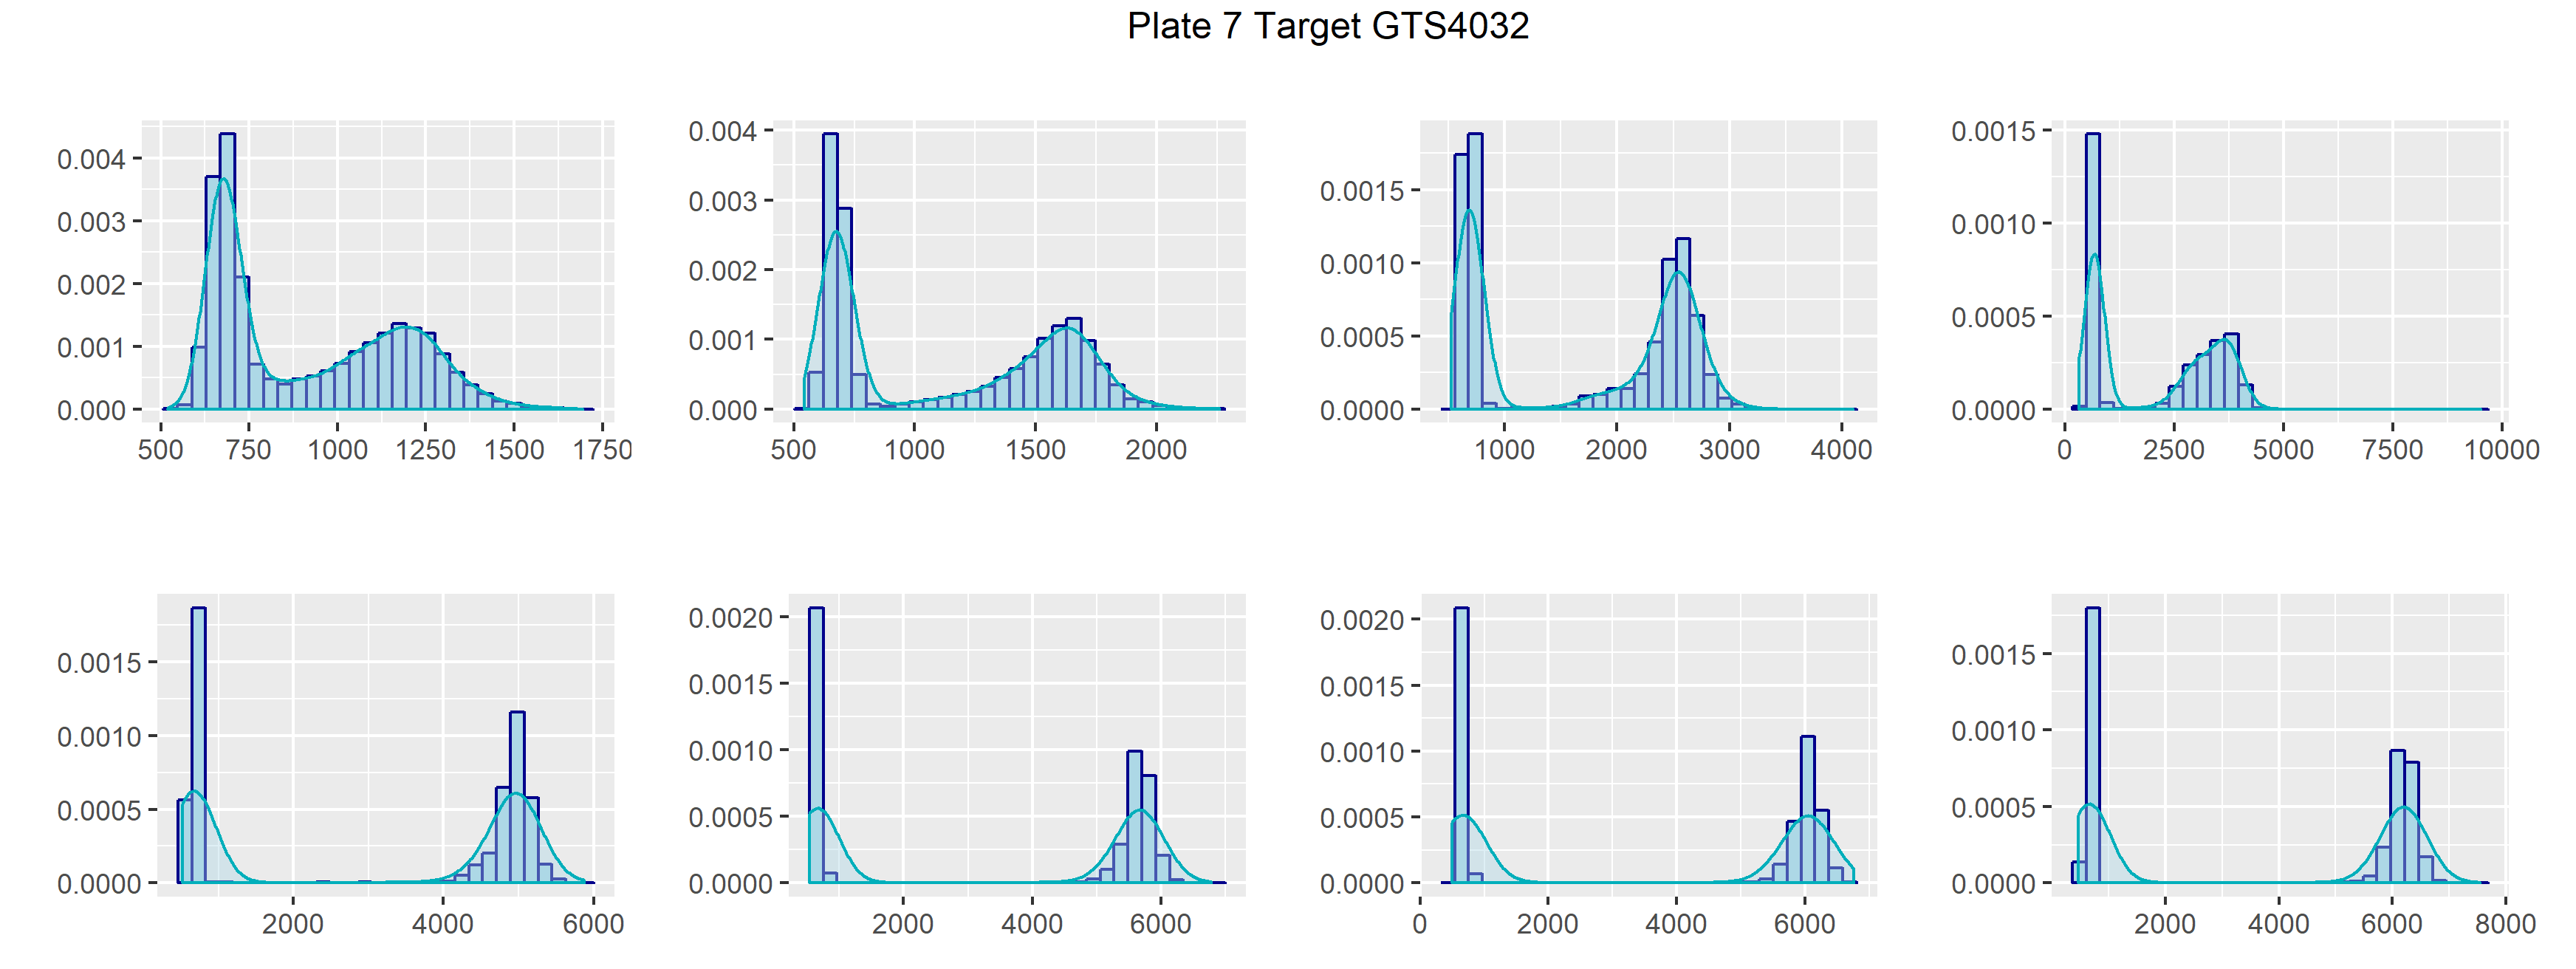
\includegraphics[max size={\textwidth}{\textheight}]{Plate 7 Target GTS4032.png}
    \caption[Target DNA GTS4032 in plate 7 of Lievens' dataset]%
    {Target DNA GTS4032 in plate 7 of Lievens' dataset- Samples A to H corresponds to the annealing temperatures 62, 61.6, 60.9, 59.8, 58.4, 57.3, 56.5, and 56 \(^{\circ}\)C.}
        \label{fig:realdata_gts}
\end{figure}

Based on equation \ref{eq:lambda}, the count of negative and positive droplets can be derived as \(N_{neg} = exp(\log{N_{tot}} - \lambda)\) and \(N_{pos} = N_{tot} - N_{neg}\). For this simulation, the total droplet count \(N_{tot}\) is fixed at 20,000 for all samples, and \(\lambda\) takes on the values of 0.1, 0.2236, 0.5, 1.118, and 2.5 target copies per droplet. 

\section{Mixture Model Fitting using EM}
\label{sec:modelfitting}

The mixture models considered for clustering droplets are the Gaussian distribution, T-distribution, and skewed-T distribution. Selection of these models are based on its numerous applications in literature and also in its availability in the R package "EMMIXskew" \cite{ref:EMMIXSkew}. However, because the the negative population in a NTC sample was rejected to follow a normal distribution \cite{ref:Trypsteen2015, ref:Jacobs2017}, Gaussian mixture model was not included in the experiments. In addition, even though GH distribution was used for model fitting for the purpose of data simulation, it was not considered here as it takes a significant amount of time to run. This downside is noted by the authors of "MixGHD" package and that code efficiency is an ongoing work. The final list of this study's proposed methods are the T-distribution and skewed-T distribution mixture models and will be abbreviated as EM-T and EM-skewT, respectively.

\section{Performance Evaluation of Quantification tools}
\label{sec:performanceeval}

The list of single-channel droplet classifier methods in literature currently includes the Bio-Rad Quantasoft software, Cloudy, ddpcRquant, definetherain, and Umbrella. The differences of these droplet classifier methods along with the EM method are summarized in Table [TABLE 3]. The accessibility of these tools are listed in Table [TABLE 4]. Among these, only the Bio-Rad Quantasoft is not open-sourced and is costly to acquire. The R source codes for Cloudy, ddpcRquant, and Umbrella is publicly accessible from the specified links. Web apps are also available for the ddpcRquant and definetherain analysis. However, not all of the methods can be used due to the resource limitations of the researcher. The final list of methods to be compared against are Cloudy, ddpcRquant, Umbrella, EM-T, and EM-skewT. 

% [ TABLE 3 ]
\begin{table}
    \caption{Table comparison of Single-channel droplet classifier methods}    
    \begin{tabularx}{\textwidth}{p{2.7cm}*{5}{X}}
        \toprule
        \textbf{Method}    & \textbf{Algorithm}                                                                                                                                                                                 & \textbf{Droplet classification rule}                                                                                                                                                            \\ 
        \midrule
        \arrayrulecolor[rgb]{0.753,0.753,0.753}
        Bio-Rad \newline QuantaSoft & (Undisclosed)                                                                                                                                            & (Undisclosed)                                                                                                                                                                                   \\
        \hline
        Cloudy                                                       & Iterative parameter estimation of \(\mu_p\) and \(\sigma_p\) using observations within the \(\hat{\mu}_p \pm a_p \cdot \hat{\sigma}_p\) of population \(p\) at each iteration.\(^1\)   & Negative if   fluorescence is \(< \hat{\mu}_{neg}+1.5 \cdot a_{neg} \cdot \hat{\sigma}_{neg}\)\\
        \hline
        ddpcRquant                                                   & Extreme Value theory to estimate negative population                                                                                                     & Negative if fluorescence is less   than the average of one hundred 0.995 percentiles of extreme values sampled                                                                                  \\
        \hline
        definetherain                                                & K-means clustering to cluster 2 populations                                                                                                              & Negative if fluorescence is \(< \hat{\mu}_{neg}   + 3 \cdot \hat{\sigma}_{neg}\); positive if fluorescence is \(> \hat{\mu}_{pos}   + 3 \cdot \hat{\sigma}_{pos}\); otherwise, droplet is rain. \\
        \hline
        Umbrella                                                     & Non-parametric approach to estimate a 2-component mixture density                                                                                        & Negative if the droplet’s probability   given the negative population is \(> 80\%\)                                                                                                             \\ 
        \hline
        EM-T / \newline EM-skewT    & Expectation Maximization to estimate a G-component mixture density                                                                                       & Droplet population membership is where its probability given a population is highest.                                                                                                           \\ 
        \arrayrulecolor{black}
        \bottomrule    
    \end{tabularx}
    {\footnotesize \(^1\) \(a_p\) is derived from Lievens et. al's own analysis of in-house data. It is calculated as \(a_p = 4.55 + 0.35 \cdot \log{(k_p)}+0.045 \cdot \log{(k_p)}^2\); where \(k_p\) is the kurtosis of the estimated population \(p\).}
\end{table}

% [ TABLE 4 ]
\bgroup
\def\arraystretch{2}%  1 is the default, change whatever you need
\begin{table}[]
    \caption{Accessibility of droplet classifier methods}
    \begin{tabularx}{\textwidth}{p{2.7cm}Xp{5.5cm}}
    \toprule
    \textbf{Method}    & \textbf{Accessibility}                 & \textbf{Included in Peformance Evaluation?} \\ 
    \midrule
    Bio-Rad QuantaSoft & Paid desktop software\(^1\)            & No \newline (not available to researcher)                                                         \\ 
    Cloudy             & R code\(^2\)                           & Yes \newline                                                                                                     \\ 
    ddpcRquant         & R code\(^3\) and free web app\(^4\)    & Yes, only in simulated data \newline (required NTC samples input are not available in Lievens’ dataset) \\ 
    definetherain      & Free web app\(^5\)                     & No \newline (required positive control samples input are not available)                                 \\ 
    Umbrella           & R code\(^6\)                           & Yes                                                                                                     \\ 
    \bottomrule
    \end{tabularx}
    {\scriptsize 
    \(^1\)https://www.bio-rad.com/en-ph/sku/1864011-quantasoft-software-regulatory-edition?ID=1864011 \newline
    \(^2\)https://github.com/Gromgorgel/ddPCR/blob/master/Cloudy-V2-05.R \newline
    \(^3\)https://ddpcrquant.ugent.be/ddpcrquant\_functions\_qx100.R \newline
    \(^4\)http://statapps.ugent.be/dPCR/ddpcrquant/\newline
    \(^5\)http://www.definetherain.org.uk/ \newline
    \(^6\)https://github.com/statOmics/umbrella/blob/master/1D/Umbrella\_1d\_V1.R
    }
\end{table}
\egroup

The estimated mean concentration per droplet \(\lambda\) will be used as the variable of interest. For the real dataset, since the real value \(\lambda\) is unknown, it is difficult to assess the method's accuracy. For this reason, the precision of \(\lambda\) estimates within sample replicates will be used as a performance metric; this is measured here using the coefficient of variation (CV). Just from the overview of the experiment setup in [TABLE 1], it is expected that the dPCR quality for all DNA targets will be different due to the varying parameters. Thus, the estimated \(\lambda\) CV of a DNA target is grouped together by the experimental levels per plate. Each level per plate and DNA target in [TABLE 1] consists of at least four technical replicates. The exceptions are plate 2, where each primer concentration only has two replicates, and plate 7, where each temperature only has one replicate. For these exceptions, the groupings would only be on the DNA targets, regardless of the experimental levels. In total, for all level and DNA target groups per plate with the exceptions, 88 CVs will be produced \footnote{Sum of level x DNA target groups for all plates, where the levels of plates 2 and 7 are combined. Then this means plates 1, 2, and 7 have \(1 \times 12\) groups; plates 3 and 6 have \(6 \times 2\) groups; plate 4 has \(3 \times 2\) groups; plate 5 has \(8 \times 2\) groups; and plate 9 has \(1 \times 10\) groups. Adding up to \(3(12) + 2(62) + (32) + (8*3) + (10) = 88\) groups.}, and to summarize these information more effectively, the distribution of the CVs will be assessed instead — first, within plates, and then within DNA targets per plate. In the case of plate 3 where a dilution series was prepared, the log-log regression model in equation [LOGLOG EQUATION] can be fitted; and for this case, in addition to CV, \(R^2\) and RSE will also be used to assess the quantification methods.

In the evaluation of methods using simulated data, since the true value of \(\lambda\) is known, then the linear regression \(\lambda = \beta_0 + \hat{\lambda}\beta_1 + \epsilon\) can be fitted. The best case scenario is that the estimated \(\hat{\lambda}\) is always equal to the true value of \(\lambda\). Thus, it is ideal that a method's \(\hat{\lambda}\) estimates will produce fitted coefficients with values very close to \(b_0=0\) and \(b_1=1\), and adequacy metrics of \(R^2=1\) and RSE=0.